% ==========================================================================
%  Make the inputs agree  --  twelve op-amp circuits on one 16:9 landscape poster
%  Same palette, type and boxes as the Ten Commandments poster; the real op-amp
%  has its own slide, the-real-mccoy.tex. Both \input preamble.tex.
%  Compile: just
% ==========================================================================
\RequirePackage{fix-cm}
\documentclass{article}
\usepackage[paperwidth=1067mm,paperheight=600mm,left=13mm,right=13mm,top=8mm,bottom=10mm]{geometry}
% ==========================================================================
%  Shared preamble for the op-amp slides (packages, palette, boxes, plot styles).
%  The top files set \documentclass and geometry, then \input this.
% ==========================================================================
\usepackage[utf8]{inputenc}
\usepackage[T1]{fontenc}
\usepackage[sc]{mathpazo}          % Palatino text + math
\linespread{1.05}
\usepackage{amsmath,amssymb,bm}
\usepackage{xcolor}
\usepackage{tikz}
\usetikzlibrary{arrows.meta,calc}
\usepackage{pgfplots}
\pgfplotsset{compat=1.16}
\usepgfplotslibrary{fillbetween}
\usepackage[siunitx,american,europeanresistors]{circuitikz}
\usepackage[most]{tcolorbox}
\usepackage[hidelinks]{hyperref}

\pagestyle{empty}
\setlength{\parindent}{0pt}

% ---------------- palette ----------------
\definecolor{paper}{HTML}{F8F5EE}
\definecolor{ink}{HTML}{1E2430}
\definecolor{accent}{HTML}{1F4E79}
\definecolor{accentlt}{HTML}{6E93B5}
\definecolor{trap}{HTML}{9A3B2E}
\definecolor{muted}{HTML}{6B7280}
\definecolor{rule}{HTML}{B9C6D3}
\definecolor{good}{HTML}{3C7A4A}
\definecolor{steel}{HTML}{D9DEE4}
\pagecolor{paper}
\color{ink}

\newcommand{\repourl}{https://github.com/samo4/ee-posters}

% ---------------- sizes ----------------
\renewcommand{\normalsize}{\fontsize{17}{21}\selectfont}
\renewcommand{\small}{\fontsize{14}{17}\selectfont}
\renewcommand{\footnotesize}{\fontsize{12.5}{15}\selectfont}
\newcommand{\eqsize}{\fontsize{19}{23}\selectfont}
\normalsize

\newcommand{\setdisplay}{%
  \setlength{\abovedisplayskip}{3pt}\setlength{\belowdisplayskip}{3pt}%
  \setlength{\abovedisplayshortskip}{3pt}\setlength{\belowdisplayshortskip}{3pt}}

% ---------------- equation group: a thin box holding equations that belong together
\newtcolorbox{eqgroup}[1][]{%
  enhanced, colback=white, colframe=rule, boxrule=0.7pt, arc=2.5mm,
  left=6pt, right=6pt, top=5pt, bottom=2pt, before skip=8pt, after skip=2pt,
  fontupper=\eqsize, before upper={\setdisplay},
  title={#1}, fonttitle=\footnotesize\scshape, coltitle=muted,
  attach boxed title to top left={xshift=4mm, yshift=-\tcboxedtitleheight/2},
  boxed title style={colback=white, colframe=white, boxrule=0pt, arc=0pt,
                     left=3pt, right=3pt, top=0pt, bottom=0pt}}
% short prose inside a box
\newcommand{\note}[1]{{\small\color{muted}#1\par}}

\newcommand{\trap}[1]{{\centering\fontsize{14.5}{17.5}\selectfont\itshape\color{trap}#1\par}}

% ---------------- card: one circuit, or one way a real op-amp falls short ----------------
% [#1] extra options, #2 name, #3 the maxim, #4 where you meet it (sits on the bottom border)
\newtcolorbox{card}[4][]{%
  enhanced, colback=white, colframe=accent, boxrule=1.4pt, arc=4mm,
  left=8pt, right=8pt, top=3pt, bottom=12pt,
  title={%
    \begin{tikzpicture}[baseline=(n.base)]
      \node[rounded corners=5mm, fill=white, text=accent, minimum height=11mm, inner xsep=3mm, inner ysep=0pt,
            font=\fontsize{23}{23}\selectfont\bfseries] (n) {#2};
    \end{tikzpicture}\par\vspace{1.5mm}
    {\fontsize{20}{24}\selectfont\bfseries\itshape #3}},
  colbacktitle=accent, coltitle=white,
  toptitle=4pt, bottomtitle=4pt, lefttitle=8pt, righttitle=8pt,
  segmentation hidden, space to upper, middle=1pt,
  overlay={\node[fill=white, draw=accent, line width=1.4pt, rounded corners=2.5mm, text width=150mm, align=center,
                 inner xsep=9pt, inner ysep=5pt, font=\small, text=ink, anchor=center]
                 at (frame.south) {#4};},
  #1}

% the schematic (left) and what it does to a signal (right)
\newcommand{\figs}[2]{%
  \begin{minipage}[c]{0.61\linewidth}\centering #1\end{minipage}\hfill
  \begin{minipage}[c]{0.38\linewidth}\centering #2\end{minipage}\par}

% ---------------- schematics ----------------
\ctikzset{bipoles/length=1.7cm, amplifiers/scale=1.45}
\tikzset{sch/.style={scale=1.12, line width=1.3pt, font=\normalsize},
         fix/.style={color=muted, dashed}}   % the part that fixes the trap

% ---------------- signals ----------------
\tikzset{vin/.style={muted, dashed, line width=1.4pt},
         vout/.style={accent, line width=1.8pt},
         vbad/.style={trap, line width=1.4pt},
         tag/.style={font=\small, inner sep=1pt}}
% over time
\pgfplotsset{wave/.style={
  scale only axis, width=46mm, height=54mm, axis lines=middle, axis line style={-{Latex[length=3mm]}, thick},
  ticks=none, label style={font=\normalsize}, xlabel={$t$},
  every axis x label/.style={at={(current axis.right of origin)}, anchor=west, xshift=1mm},
  samples=300, domain=0:720, xmin=0, xmax=760, clip=false}}
% output over input
\pgfplotsset{xfer/.style={
  scale only axis, width=44mm, height=54mm, axis lines=middle, clip=false, axis line style={-{Latex[length=3mm]}, thick},
  tick style={draw=none}, ticklabel style={font=\small}, label style={font=\normalsize},
  xlabel={$v_\text{in}$}, ylabel={$v_\text{out}$},
  every axis x label/.style={at={(current axis.right of origin)}, anchor=west, xshift=1mm},
  every axis y label/.style={at={(current axis.above origin)}, anchor=south},
  every axis plot/.append style={line width=1.8pt}}}
% level in dB over frequency
\pgfplotsset{bode/.style={
  scale only axis, width=50mm, height=54mm, axis x line=bottom, clip=false, axis y line=left,
  axis line style={-{Latex[length=3mm]}, thick}, tick style={draw=none}, ticklabel style={font=\small},
  label style={font=\normalsize}, xlabel={$f$},
  every axis x label/.style={at={(axis description cs:1,0)}, anchor=west, xshift=1mm},
  samples=200, every axis plot/.append style={line width=1.8pt}}}
% second-order low-pass magnitude, x = f/f_0
\pgfmathdeclarefunction{lp}{2}{\pgfmathparse{1/sqrt((1-#1^2)^2+(#1/#2)^2)}}
% triangle and square waves of x in degrees, amplitude 1, both rising through 0 at x = 0
\pgfmathdeclarefunction{tri}{1}{\pgfmathparse{asin(sin(#1))/90}}
\pgfmathdeclarefunction{sqr}{1}{\pgfmathparse{sin(#1)>=0 ? 1 : -1}}

% a column that fills the page height; \vfill between blocks spreads them out
\newenvironment{pagecol}[1]{\begin{minipage}[t][\dimexpr\textheight-\topskip\relax][s]{#1}\vspace{0pt}}{\end{minipage}}



\begin{document}
\noindent
% gutter notes, read top to bottom: the legend and a quip down the left edge,
% the next slide and the repository down the right edge
\begin{tikzpicture}[remember picture, overlay]
  \begin{scope}[shift={($(current page.west)+(6.3mm,0mm)$)}, rotate=-90, transform shape, x=1mm, y=1mm,
                every node/.style={anchor=west, font=\fontsize{17}{20}\selectfont, text=ink}]
    \draw[vin] (-265,0) -- (-253,0) node[right=2mm] {$v_\text{in}$};
    \draw[vout] (-225,0) -- (-213,0) node[right=2mm] {$v_\text{out}$};
    \draw[vbad] (-183,0) -- (-171,0) node[right=2mm] {what goes wrong};
    \draw[muted, dashed, line width=1.3pt] (-110,0) -- (-98,0) node[right=2mm] {the fix};
    \node[anchor=center, text=trap, font=\fontsize{17}{20}\selectfont\itshape] at (110,0)
      {\upshape\bfseries Puzzle:\mdseries\itshape\ what happens if you replace the capacitor in the integrator with an inductor?};
  \end{scope}
  \node[rotate=-90, anchor=center, text=muted, font=\fontsize{14}{17}\selectfont\itshape]
    at ($(current page.east)+(-6.3mm,0mm)$)
    {The ideal op-amp, and the dozen ways a real one falls short of it:
     \upshape\bfseries\color{accent}The real McCoy, on the next slide.\quad
     \mdseries\href{\repourl}{\color{accent}\repourl}};
\end{tikzpicture}%
% ===================================================================== title, across the page
{\fontsize{28}{32}\selectfont\scshape\color{muted} Op-amp circuits, or:}\enspace
{\fontsize{72}{76}\selectfont\bfseries Make the inputs agree}\hfill
{\fontsize{23}{28}\selectfont\color{muted}\itshape
 The output does whatever it takes to hold $v_+=v_-$.\quad
 \upshape\bfseries\color{trap} Gain $\times$ bandwidth is a constant. Spend it.}\par
\vspace{3mm}
{\color{accent}\rule{\linewidth}{2.5pt}}\par
\vspace{6mm}
% ===================================================================== twelve circuits, across the page
\noindent
\begin{minipage}[t]{\linewidth}\vspace{0pt}
\begin{tcbraster}[raster columns=4, raster equal height=rows, raster column skip=7mm, raster row skip=15mm,
                  raster force size=false]
% ---------------------------------------------------------------- voltage follower
\begin{card}[height=169mm, valign upper=center]{Voltage follower}{Copy the voltage; supply the current.}%
  {Reference and ADC buffers, sensors with a high source impedance.}
\figs{%
  \begin{circuitikz}[sch]
    \node[op amp, noinv input up] (A) at (0,0) {};
    \draw (A.+) to[short, -o] ++(-1.4,0) node[left] {$v_\text{in}$};
    \draw (A.out) to[short, -*] ++(0.6,0) coordinate (o) to[short, -o] ++(0.9,0) node[above] {$v_\text{out}$};
    \draw (A.-) -- ++(-0.5,0) |- ($(o)+(0,-2)$) -- (o);
  \end{circuitikz}}{%
  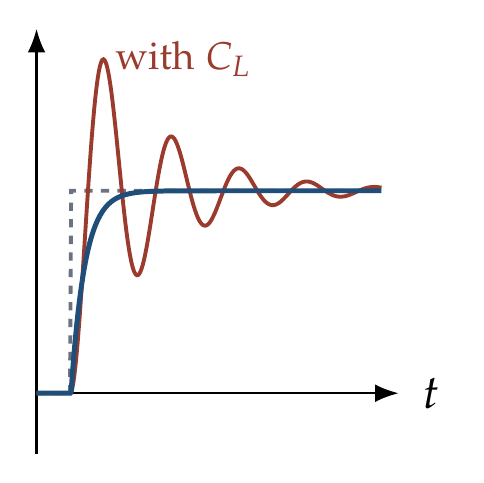
\begin{tikzpicture}
  \begin{axis}[wave, domain=0:10, xmin=0, xmax=10.5, ymin=-0.3, ymax=1.8]
    \addplot[vin] {x<1 ? 0 : 1};
    \addplot[vbad] {x<1 ? 0 : 1-exp(-0.45*(x-1))*cos(deg(3.2*(x-1)))};
    \addplot[vout] {x<1 ? 0 : 1-exp(-2.5*(x-1))};
    \node[tag, text=trap, anchor=west] at (axis cs:2.2,1.65) {with $C_L$};
  \end{axis}
  \end{tikzpicture}}
\begin{eqgroup}[Gain one; the loop transforms the impedances]
\[ v_\text{out}=v_\text{in}\qquad Z_\text{out}\approx\frac{r_o}{1+A} \]
\note{The source sees gigaohms, the load sees milliohms. A buffer is a voltage copied into a stiffer source.}
\end{eqgroup}
\tcblower
\trap{\textbf{Unity gain has the least phase margin.} A cable or a capacitive load makes it ring; isolate it with a few ohms in series.}
\end{card}
% ---------------------------------------------------------------- non-inverting
\begin{card}[height=169mm, valign upper=center]{Non-inverting}{Gain without loading the source.}%
  {Sensor and microphone preamps, ADC gain stages.}
\figs{%
  \begin{circuitikz}[sch]
    \node[op amp, noinv input up] (A) at (0,0) {};
    \draw (A.+) to[short, -o] ++(-1.4,0) node[left] {$v_\text{in}$};
    \draw (A.out) to[short, -*] ++(0.6,0) coordinate (o) to[short, -o] ++(0.9,0) node[above] {$v_\text{out}$};
    \draw (A.-) -- ++(-0.5,0) coordinate (n) -- ++(0,-1.2) coordinate (b) to[R, l_=$R_f$, *-] (b -| o) -- (o);
    \draw (b) to[R, l_=$R_g$] ++(0,-1.7) node[tground] {};
  \end{circuitikz}}{%
  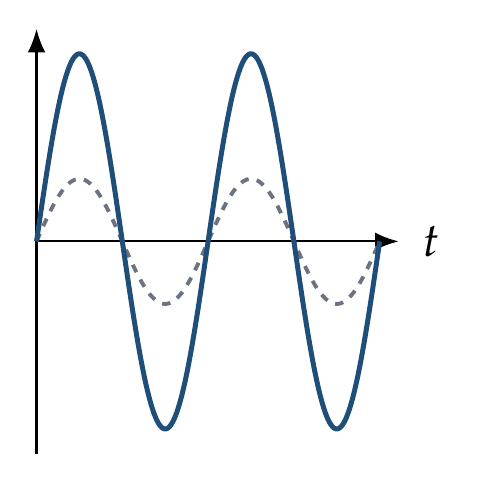
\begin{tikzpicture}
  \begin{axis}[wave, ymin=-1.7, ymax=1.7]
    \addplot[vin] {0.5*sin(x)};
    \addplot[vout] {1.5*sin(x)};
  \end{axis}
  \end{tikzpicture}}
\begin{eqgroup}[Signal gain equals noise gain]
\[ v_\text{out}=\Bigl(1+\frac{R_f}{R_g}\Bigr)\,v_\text{in} \]
\note{Input impedance is the op-amp's own, gigaohms. The gain can never drop below 1.}
\end{eqgroup}
\tcblower
\trap{\textbf{Both inputs ride on $v_\text{in}$.} Check the input common-mode range, not only the output swing.}
\end{card}
% ---------------------------------------------------------------- inverting
\begin{card}[height=169mm, valign upper=center]{Inverting}{Hold the input at a virtual ground.}%
  {Gain stages, active filters, level shifts.}
\figs{%
  \begin{circuitikz}[sch]
    \node[op amp] (A) at (0,0) {};
    \draw (A.-) -- ++(-0.5,0) coordinate (n);
    \draw ($(n)+(-2.1,0)$) node[left] {$v_\text{in}$} to[R, l=$R_\text{in}$, o-*] (n);
    \draw (A.out) to[short, -*] ++(0.6,0) coordinate (o) to[short, -o] ++(0.9,0) node[below] {$v_\text{out}$};
    \draw (n) -- ++(0,1.5) coordinate (t) to[R, l=$R_f$] (t -| o) -- (o);
    \draw (A.+) -- ++(-0.4,0) -- ++(0,-0.3) node[tground] {};
  \end{circuitikz}}{%
  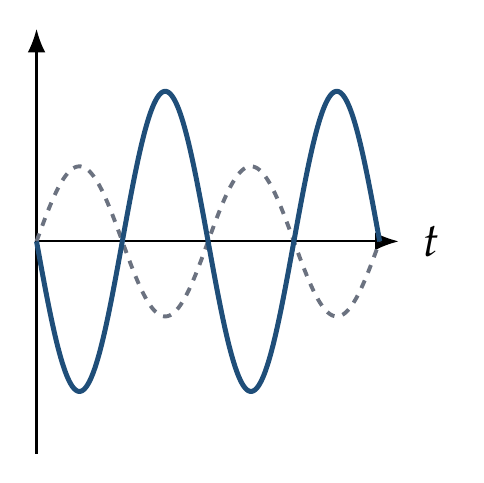
\begin{tikzpicture}
  \begin{axis}[wave, ymin=-1.7, ymax=1.7]
    \addplot[vin] {0.6*sin(x)};
    \addplot[vout] {-1.2*sin(x)};
  \end{axis}
  \end{tikzpicture}}
\begin{eqgroup}[The source drives a resistor to ground]
\[ v_\text{out}=-\frac{R_f}{R_\text{in}}\,v_\text{in}\qquad Z_\text{in}=R_\text{in} \]
\note{$v_-$ sits at 0\,V, so the inputs never see a common-mode swing, and the gain may be below 1.}
\end{eqgroup}
\tcblower
\trap{\textbf{Bandwidth follows the noise gain $1+R_f/R_\text{in}$:} a gain of $-1$ is as slow as $+2$.}
\end{card}
% ---------------------------------------------------------------- summing
\begin{card}[height=169mm, valign upper=center]{Summing}{Currents meet at the virtual ground.}%
  {Audio mixers, weighted DACs, offset injection.}
\figs{%
  \begin{circuitikz}[sch]
    \node[op amp] (A) at (0,0) {};
    \draw (A.-) -- ++(-0.5,0) coordinate (n);
    \draw (A.out) to[short, -*] ++(0.6,0) coordinate (o) to[short, -o] ++(0.9,0) node[below] {$v_\text{out}$};
    \foreach \i/\y in {3/0, 2/1.3, 1/2.6}
      \draw ($(n)+(-2.1,\y)$) node[left] {$v_\i$} to[R, l=$R_\i$, o-*] ($(n)+(0,\y)$);
    \draw (n) -- ++(0,3.9) coordinate (t) to[R, l=$R_f$] (t -| o) -- (o);
    \draw (A.+) -- ++(-0.4,0) -- ++(0,-0.3) node[tground] {};
  \end{circuitikz}}{%
  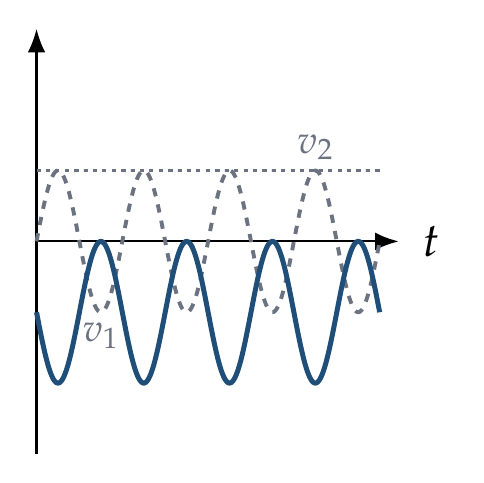
\begin{tikzpicture}
  \begin{axis}[wave, ymin=-1.5, ymax=1.5]
    \addplot[vin] {0.5*sin(2*x)};
    \addplot[vin, dotted] {0.5};
    \addplot[vout] {-(0.5*sin(2*x)+0.5)};
    \node[tag, text=muted, anchor=south west] at (axis cs:540,0.55) {$v_2$};
    \node[tag, text=muted, anchor=north] at (axis cs:135,-0.55) {$v_1$};
  \end{axis}
  \end{tikzpicture}}
\begin{eqgroup}[Each input sends its own current into $R_f$]
\[ v_\text{out}=-R_f\Bigl(\frac{v_1}{R_1}+\frac{v_2}{R_2}+\frac{v_3}{R_3}\Bigr) \]
\note{The virtual ground keeps the inputs from talking to each other. Weight them $1,2,4,\ldots$ and it is a DAC.}
\end{eqgroup}
\tcblower
\trap{\textbf{Every input you add raises the noise gain $1+R_f/(R_1\|R_2\|R_3)$:} bandwidth and noise, for all of them.}
\end{card}
% ---------------------------------------------------------------- difference
\begin{card}[height=169mm, valign upper=center]{Difference}{Amplify what differs; reject what is shared.}%
  {Current-shunt sensing, balanced line receivers.}
\figs{%
  \begin{circuitikz}[sch]
    \node[op amp] (A) at (0,0) {};
    \draw (A.-) -- ++(-0.5,0) coordinate (n);
    \draw (A.+) -- ++(-0.5,0) coordinate (p);
    \draw ($(n)+(-2.1,0)$) node[left] {$v_1$} to[R, l=$R_1$, o-*] (n);
    \draw ($(p)+(-2.1,0)$) node[left] {$v_2$} to[R, l_=$R_3$, o-*] (p);
    \draw (A.out) to[short, -*] ++(0.6,0) coordinate (o) to[short, -o] ++(0.9,0) node[below] {$v_\text{out}$};
    \draw (n) -- ++(0,1.5) coordinate (t) to[R, l=$R_2$] (t -| o) -- (o);
    \draw (p) to[R, l=$R_4$] ++(0,-1.7) node[tground] {};
  \end{circuitikz}}{%
  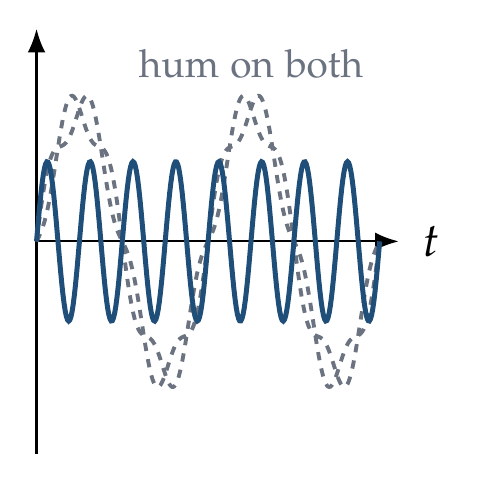
\begin{tikzpicture}
  \begin{axis}[wave, ymin=-1.6, ymax=1.6]
    \addplot[vin] {sin(x)+0.15*sin(4*x)};
    \addplot[vin] {sin(x)-0.15*sin(4*x)};
    \addplot[vout] {0.6*sin(4*x)};
    \node[tag, text=muted, anchor=south] at (axis cs:450,1.2) {hum on both};
  \end{axis}
  \end{tikzpicture}}
\begin{eqgroup}[Balanced when $R_4/R_3=R_2/R_1$; $t$ is the resistor tolerance]
\[ v_\text{out}=\frac{R_2}{R_1}\,(v_2-v_1) \]
\[ \text{CMRR}\gtrsim\frac{1+R_2/R_1}{4\,t} \]
\end{eqgroup}
\tcblower
\trap{\textbf{1\,\% resistors give 34\,dB at unity gain,} and the source impedance joins the bridge. Buy a matched network, preferably with opamp attached.}
\end{card}
% ---------------------------------------------------------------- instrumentation
\begin{card}[height=169mm, valign upper=center]{Instrumentation}{Buffer both inputs, then subtract.}%
  {Strain-gauge bridges, ECG, thermocouples.}
{\centering
  \begin{circuitikz}[sch, scale=1]
    \node[op amp, noinv input up] (A1) at (0,2.6) {};
    \node[op amp] (A2) at (0,-2.6) {};
    \node[op amp] (A3) at (9.5,0) {};
    \draw (A1.+) to[short, -o] ++(-1,0) node[left] {$v_1$};
    \draw (A2.+) to[short, -o] ++(-1,0) node[left] {$v_2$};
    \draw (A1.out) to[short, -*] ++(0.8,0) coordinate (o1);
    \draw (A2.out) to[short, -*] ++(0.8,0) coordinate (o2);
    \draw (A1.-) -- ++(-0.6,0) coordinate (n1) -- ++(0,-0.9) coordinate (c1);
    \draw (A2.-) -- ++(-0.6,0) coordinate (n2) -- ++(0,0.9) coordinate (c2);
    \draw (c1) to[R, l=$R$, *-] (c1 -| o1) -- (o1);
    \draw (c2) to[R, l_=$R$, *-] (c2 -| o2) -- (o2);
    \draw (c1) to[R, l_=$R_G$, color=accent] (c2);
    \draw (A3.-) -- ++(-0.5,0) coordinate (m);
    \draw (A3.+) -- ++(-0.5,0) coordinate (q);
    \draw (o1) -- ++(0.8,0) |- ($(m)+(-2.2,0)$) to[R, l=$R$, -*] (m);
    \draw (o2) -- ++(0.8,0) |- ($(q)+(-2.2,0)$) to[R, l_=$R$, -*] (q);
    \draw (A3.out) to[short, -*] ++(0.6,0) coordinate (o) to[short, -o] ++(0.9,0) node[below] {$v_\text{out}$};
    \draw (m) -- ++(0,1.8) coordinate (t) to[R, l=$R$] (t -| o) -- (o);
    \draw (q) to[R, l=$R$] ++(0,-1.9) node[tground] {};
  \end{circuitikz}\par}
\begin{eqgroup}[Every resistor the same $R$, but one: $R_G$ sets the gain]
\[ v_\text{out}=\Bigl(1+\frac{2R}{R_G}\Bigr)\,(v_2-v_1) \]
\end{eqgroup}
\tcblower
\trap{\textbf{Inner nodes saturate while the output looks fine.} Check the datasheet's common-mode ``diamond''.}
\end{card}
% ---------------------------------------------------------------- transimpedance
\begin{card}[height=169mm, valign upper=center]{Transimpedance}{Turn a current into a voltage, at zero volts.}%
  {Photodiodes, lidar, current-output DACs.}
\figs{%
  \begin{circuitikz}[sch]
    \node[op amp] (A) at (0,0) {};
    \draw (A.-) -- ++(-0.5,0) coordinate (n);
    \draw (A.out) to[short, -*] ++(0.6,0) coordinate (o) to[short, -o] ++(0.9,0) node[below] {$v_\text{out}$};
    \draw (n) to[short, *-] ++(-1,0) coordinate (d);
    \draw (d) ++(0,-2) node[tground] {} to[pD, l=$C_\text{in}$] (d);
    \draw (n) -- ++(0,1.4) coordinate (t) to[R, l=$R_f$] (t -| o) -- (o);
    \draw (t) to[short, *-] ++(0,1.7) coordinate (t2) to[C, l=$C_f$, fix] (t2 -| o) to[short, -*] (t -| o);
    \draw (A.+) -- ++(-0.4,0) -- ++(0,-0.3) node[tground] {};
  \end{circuitikz}}{%
  \begin{tikzpicture}
  \begin{semilogxaxis}[bode, width=48mm, xmin=0.05, xmax=20, ymin=-30, ymax=14, domain=0.05:20, restrict y to domain=-30:14,
      xtick={1}, xticklabels={$f_{-3\,\text{dB}}$}, ytick={0}, yticklabels={$R_f$}]
    \draw[muted, dashed, line width=0.8pt] (axis cs:0.05,0) -- (axis cs:20,0);
    \addplot[vbad] {20*log10(lp(x,3))};
    \addplot[vout] {20*log10(lp(x,0.707))};
    \node[tag, text=trap, anchor=south] at (axis cs:1,10.5) {no $C_f$};
  \end{semilogxaxis}
  \end{tikzpicture}}
\begin{eqgroup}[$v_\text{out}=i_\text{ph}R_f$; the photodiode's $C_\text{in}$ sits in the loop]
\[ f_{-3\,\text{dB}}\approx\sqrt{\frac{\text{GBW}}{2\pi R_fC_\text{in}}}\qquad C_f\approx\sqrt{\frac{C_\text{in}}{2\pi R_f\,\text{GBW}}} \]
\end{eqgroup}
\tcblower
\trap{\textbf{Without $C_f$ the diode's capacitance adds a pole in the loop:} it rings, or it oscillates.}
\end{card}
% ---------------------------------------------------------------- logarithmic
\begin{card}[height=169mm, valign upper=center]{Logarithmic}{Put an exponential in the loop; get its inverse.}%
  {RF power detectors, dB meters, analog multipliers.}
\figs{%
  \begin{circuitikz}[sch]
    \node[op amp] (A) at (0,0) {};
    \draw (A.-) -- ++(-0.5,0) coordinate (n);
    \draw ($(n)+(-2.1,0)$) node[left] {$v_\text{in}$} to[R, l=$R$, o-*] (n);
    \draw (A.out) to[short, -*] ++(0.6,0) coordinate (o) to[short, -o] ++(0.9,0) node[below] {$v_\text{out}$};
    \draw (n) -- ++(0,1.5) coordinate (t) to[D, l=$D$] (t -| o) -- (o);
    \draw (A.+) -- ++(-0.4,0) -- ++(0,-0.3) node[tground] {};
  \end{circuitikz}}{%
  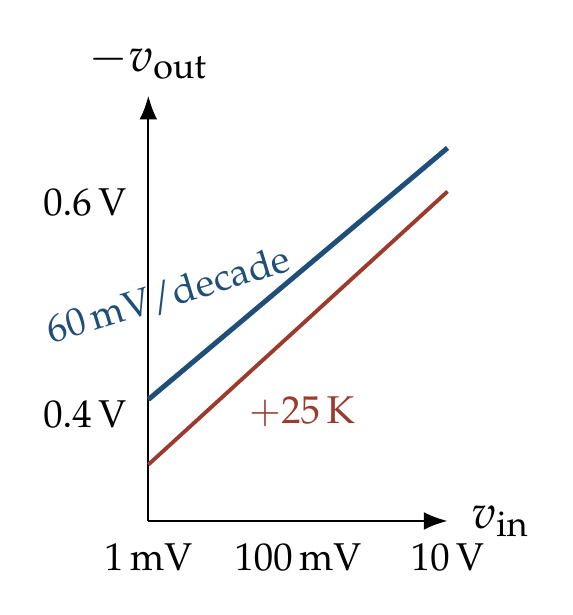
\begin{tikzpicture}
  \begin{semilogxaxis}[bode, width=38mm, xmin=1e-3, xmax=10, ymin=0.3, ymax=0.7, domain=1e-3:10,
      xlabel={$v_\text{in}$}, ylabel={$-v_\text{out}$},
      every axis y label/.style={at={(axis description cs:0,1)}, anchor=south},
      xtick={1e-3,1e-1,10}, xticklabels={1\,mV,100\,mV,10\,V}, ytick={0.4,0.6}, yticklabels={0.4\,V,0.6\,V}]
    \addplot[vbad] {0.0279*ln(x*3.125e8)};
    \addplot[vout] {0.0257*ln(x*1e10)};
    \node[tag, text=accent, anchor=south east, rotate=17] at (axis cs:0.1,0.53) {60\,mV/decade};
    \node[tag, text=trap, anchor=north west] at (axis cs:0.02,0.42) {$+25$\,K};
  \end{semilogxaxis}
  \end{tikzpicture}}
\begin{eqgroup}[The diode's $i=I_S\,e^{v/V_T}$, turned inside out]
\[ v_\text{out}=-V_T\ln\frac{v_\text{in}}{R\,I_S} \]
\note{$V_T\ln10=59.5$\,mV per decade at 300\,K: six decades of input in 360\,mV. Positive inputs only.}
\end{eqgroup}
\tcblower
\trap{\textbf{$V_T$ and $I_S$ both drift with temperature.} Real log amps cancel $I_S$ with a matched transistor.}
\end{card}
% ---------------------------------------------------------------- integrator
\begin{card}[height=169mm, valign upper=center]{Integrator}{Charge a capacitor with a current you set.}%
  {PID's I-term, ramp generators, dual-slope ADCs.}
\figs{%
  \begin{circuitikz}[sch]
    \node[op amp] (A) at (0,0) {};
    \draw (A.-) -- ++(-0.5,0) coordinate (n);
    \draw ($(n)+(-2.1,0)$) node[left] {$v_\text{in}$} to[R, l=$R$, o-*] (n);
    \draw (A.out) to[short, -*] ++(0.6,0) coordinate (o) to[short, -o] ++(0.9,0) node[below] {$v_\text{out}$};
    \draw (n) -- ++(0,1.4) coordinate (t) to[C, l=$C$] (t -| o) -- (o);
    \draw (t) to[short, *-] ++(0,1.7) coordinate (t2) to[R, l=$R_p$, fix] (t2 -| o) to[short, -*] (t -| o);
    \draw (A.+) -- ++(-0.4,0) -- ++(0,-0.3) node[tground] {};
  \end{circuitikz}}{%
  \begin{tikzpicture}
  \begin{axis}[wave, ymin=-1.5, ymax=1]
    \addplot[vin] {0.5*sqr(x)};
    \addplot[vout] {-0.6*(1-asin(cos(x))/90)};
  \end{axis}
  \end{tikzpicture}}
\begin{eqgroup}[The input current $v_\text{in}/R$ charges $C$]
\[ v_\text{out}=-\frac{1}{RC}\int_0^t v_\text{in}\,d\tau\qquad H(s)=-\frac{1}{sRC} \]
\note{Infinite gain at DC; $R_p$ limits it to $-R_p/R$ below $1/(2\pi R_pC)$.}
\end{eqgroup}
\tcblower
\trap{\textbf{Offset and bias current integrate too.} Without $R_p$ or a reset switch, it walks to the rail.}
\end{card}
% ---------------------------------------------------------------- differentiator
\begin{card}[height=169mm, valign upper=center]{Differentiator}{Measure how fast it changes.}%
  {Filtered PID D-terms, edge and rate detectors.}
\figs{%
  \begin{circuitikz}[sch]
    \node[op amp] (A) at (0,0) {};
    \draw (A.-) -- ++(-0.5,0) coordinate (n);
    \ctikzset{bipoles/length=1.2cm}
    \draw ($(n)+(-2.2,0)$) node[left] {$v_\text{in}$} to[R, l=$R_s$, fix, o-] ++(1.15,0) to[C, l=$C$, -*] (n);
    \ctikzset{bipoles/length=1.7cm}
    \draw (A.out) to[short, -*] ++(0.6,0) coordinate (o) to[short, -o] ++(0.9,0) node[below] {$v_\text{out}$};
    \draw (n) -- ++(0,1.5) coordinate (t) to[R, l=$R$] (t -| o) -- (o);
    \draw (A.+) -- ++(-0.4,0) -- ++(0,-0.3) node[tground] {};
  \end{circuitikz}}{%
  \begin{tikzpicture}
  \begin{axis}[wave, ymin=-1.1, ymax=1.1, samples=721]
    \addplot[vin] {0.8*tri(x)};
    \addplot[vout] {cos(x)>=0 ? -0.5 : 0.5};
  \end{axis}
  \end{tikzpicture}}
\begin{eqgroup}[The capacitor current $C\,dv/dt$ flows through $R$]
\[ v_\text{out}=-RC\,\frac{dv_\text{in}}{dt}\qquad H(s)=-sRC \]
\note{$R_s$ caps the gain at $-R/R_s$ above $1/(2\pi R_sC)$.}
\end{eqgroup}
\tcblower
\trap{\textbf{Its gain rises 20\,dB/decade into the op-amp's roll-off:} noise is amplified, and the loop rings. Add $R_s$.}
\end{card}
% ---------------------------------------------------------------- comparator
\begin{card}[height=169mm, valign upper=center]{Comparator}{Feed back positively; the output picks a rail.}%
  {Zero-crossing detectors, relaxation oscillators, threshold trips.}
\figs{%
  \begin{circuitikz}[sch]
    \node[op amp] (A) at (0,0) {};
    \draw (A.-) to[short, -o] ++(-1,0) node[left] {$v_\text{in}$};
    \draw (A.out) to[short, -*] ++(0.6,0) coordinate (o) to[short, -o] ++(0.9,0) node[above] {$v_\text{out}$};
    \draw (A.+) -- ++(-0.5,0) -- ++(0,-1.2) coordinate (b) to[R, l_=$R_2$, *-] (b -| o) -- (o);
    \draw (b) to[R, l_=$R_1$] ++(0,-1.7) node[tground] {};
  \end{circuitikz}}{%
  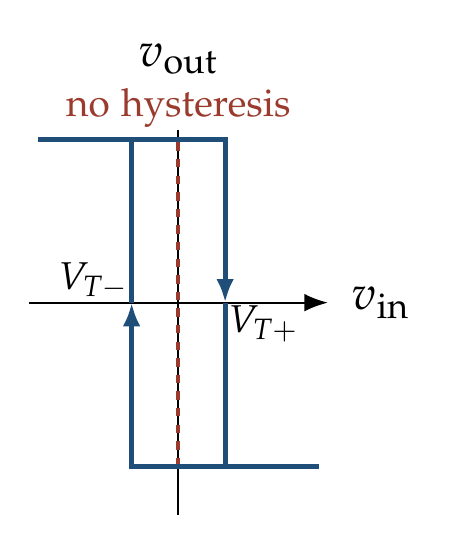
\begin{tikzpicture}
  \begin{axis}[xfer, width=38mm, xmin=-1.6, xmax=1.6, ymin=-1.3, ymax=1.3,
      xtick=\empty, ytick=\empty]
    \node[tag, anchor=north west] at (axis cs:0.5,0) {$V_{T+}$};
    \node[tag, anchor=south east] at (axis cs:-0.5,0) {$V_{T-}$};
    \addplot[vbad, dashed] coordinates {(0,-1) (0,1)};
    \addplot[vout, -{Latex[length=3mm]}] coordinates {(-1.5,1) (0.5,1) (0.5,0)};
    \addplot[vout] coordinates {(0.5,0) (0.5,-1) (1.5,-1)};
    \addplot[vout, -{Latex[length=3mm]}] coordinates {(1.5,-1) (-0.5,-1) (-0.5,0)};
    \addplot[vout] coordinates {(-0.5,0) (-0.5,1)};
    \node[tag, text=trap, anchor=south, fill=white] at (axis cs:0,1.05) {no hysteresis};
  \end{axis}
  \end{tikzpicture}}
\begin{eqgroup}[Schmitt trigger: the threshold moves with the output]
\[ V_{T\pm}=\pm\frac{R_1}{R_1+R_2}\,V_\text{sat} \]
\note{Noise smaller than the gap $V_{T+}-V_{T-}$ can no longer make the output chatter.}
\end{eqgroup}
\tcblower
\trap{\textbf{An op-amp is a slow comparator:} it recovers from saturation in microseconds, and some clamp their inputs.}
\end{card}
% ---------------------------------------------------------------- precision rectifier
\begin{card}[height=169mm, valign upper=center]{Precision rectifier}{Hide the diode's drop inside the loop.}%
  {AC voltmeters, envelope and peak detectors.}
\figs{%
  \begin{circuitikz}[sch]
    \node[op amp, noinv input up] (A) at (0,0) {};
    \draw (A.+) to[short, -o] ++(-1.2,0) node[left] {$v_\text{in}$};
    \draw (A.out) to[D, l=$D$, -*] ++(1.6,0) coordinate (k) -- ++(0.6,0) coordinate (r)
      to[short, *-o] ++(0.6,0) node[above] {$v_\text{out}$};
    \draw (r) to[R, l=$R_L$] ++(0,-2.6) node[tground] {};
    \draw (A.-) -- ++(-0.5,0) |- ($(k)+(0,-2)$) -- (k);
  \end{circuitikz}}{%
  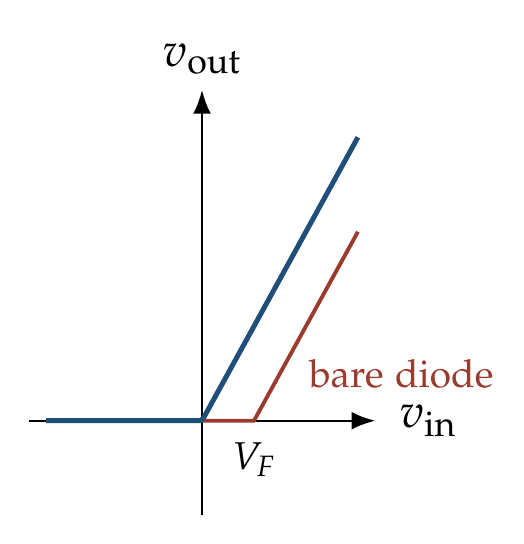
\begin{tikzpicture}
  \begin{axis}[xfer, xmin=-2, xmax=2, ymin=-0.6, ymax=2.1, domain=-1.8:1.8, samples=100,
      xtick={0.6}, xticklabels={$V_F$}, ytick=\empty]
    \addplot[vbad] {max(x-0.6,0)};
    \addplot[vout] {max(x,0)};
    \node[tag, text=trap, anchor=west] at (axis cs:1.2,0.3) {bare diode};
  \end{axis}
  \end{tikzpicture}}
\begin{eqgroup}[A superdiode: the loop divides $V_F$ by the open-loop gain]
\[ v_\text{out}=\max(v_\text{in},0)\qquad V_{F,\text{eff}}\approx\frac{V_F}{A} \]
\end{eqgroup}
\tcblower
\trap{\textbf{When the diode turns off, the loop opens} and the output slams to the rail. Recovery limits it to audio.}
\end{card}
\end{tcbraster}
\end{minipage}
\end{document}
